\section{Regulator liniowo-kwadratowy}

Po weryfikacji modelu, równania zostały zlinearyzowane. Przyjęto kilka punktów równowagi: 12mm, 14mm, 16mm i 18mm, aby móc przełączać otrzymany później regulator podczas pracy układu i stabilizować go w różnych punktach pracy.

\subsection{Linearyzacja}

Linearyzacji modelu nieliniowego dokonuje się w otoczeniu punktu równowagi, zastępując nieliniowe równania stanu
\begin{equation}
\dot{x} = f(x)
\end{equation}
liniowymi równaniami, które można przedstawić w postaci macierzowej
\begin{equation}
\dot{x} = Ax + Bu
\end{equation}

Aby otrzymać macierz stanu A, należy wyznaczyć macierz Jacobiego pierwszych pochodnych
\begin{equation}
J = \dfrac{\partial f}{\partial x}(x)
\end{equation}
a następnie obliczyć jej wartości dla poszczególnych punktów stacjonarnych $x*$
\begin{equation}
A = J(x*) = \dfrac{\partial f}{\partial x}(x*)
\end{equation}

Dla równań magnetycznej lewitacji (\ref{modelMagLev}) zlinearyzowana macierz ma postać

\[
\begin{array}{lc}
A = &
\begin{bmatrix} 0 & 1 & 0 \\ \dfrac{2 \cdot 10^{-3} agx_3^2}{(ax_1+b)^3} & 0 & \dfrac{-2 \cdot 10^{-3} gx_3}{(ax_1+b)^2} \\ 0 & 0 & -\dfrac{1}{T}
\end{bmatrix}
\end{array}
\]

W punkcie równowagi $ x_{0_{14}} = \begin{bmatrix} 0,014 \\
0 \\
0,024
\end{bmatrix}
$ macierz stanu i wektor sterowań przyjmują wartości
\[
\begin{array}{lc}
A = &
\begin{bmatrix} 0 & 1 & 0 \\
0,0897 & 0 & -0,9139 \\
0 & 0 & -41,6667
\end{bmatrix}
\\
B = & \begin{bmatrix}
0 \\ 0 \\ 10,8625
\end{bmatrix}
\end{array}
\]

\subsection{Synteza regulatora LQ}

Regulator liniowo-kwadratowy dla nieskończonego horyzontu czasowego to liniowy regulator od całego stanu, który sterowaniem
\begin{equation}
u = -Kx
\end{equation}
Sprowadza zlinearyzowany układ do zerowego punktu równowagi. Minimalizuje przy tym funkcję celu
\begin{equation}
J = \dfrac{1}{2} \int _0^{\infty} {x^T Q x + u^T R u}\: dt
\end{equation}

Macierz $K$ jest dana wzorem
\begin{equation}
K = R^{-1}B^T P
\end{equation}
gdzie $P$ to rozwiązanie algebraicznego równania Riccatiego
\begin{equation}
A^T P + PA -PBR^{-1}B^T P + Q = 0
\end{equation}

Dla macierzy wag
\[
\begin{array}{lc}
Q = &
\begin{bmatrix} 4 & 0 & 0 \\
0 & 1 & 0 \\
0 & 0 & 1
\end{bmatrix}
\\
R = & \begin{bmatrix}
1
\end{bmatrix}
\end{array}
\]
    
Macierz regulatora optymalnego LQ została obliczona jako:
\[
\begin{array}{lc}
K = &
\begin{bmatrix}
 -2,4362 \\  -4,7518  \\  0,2278
\end{bmatrix}
\end{array}
\]

Powstały układ zamknięty charakteryzuje się wartościami własnymi
\[
\begin{array}{lc}
E = eig(A-BK) &
\begin{bmatrix}
  -43,058 \\
  -0,5413 + 0,4204i \\
  -0,5413 - 0,4204i
\end{bmatrix}
\end{array}
\]

Jak wspomniano na początku rozdziału, chcemy stabilizować układ w niezerowych punktach równowagi, gdzie sterowanie ma pewną ustaloną, niezerową wartość. W tym celu używamy prawa sterowania zaczerpniętego z pracy \cite{ReferenceTrackLQR}
\begin{equation}
u = -Kx + Lr
\end{equation}
gdzie $r$ jest wartością zadaną, a $L$ macierzą wag wartości zadanej.

Stabilizacja modelu z regulatorem LQR dla linearyzacji w punkcie równowagi $ x_{0_{14}} = \begin{bmatrix} 0,014 \\
0 \\
0,024
\end{bmatrix}
$ została przedstawiona na wykresie \ref{img:model_LQR}.

\begin{figure}[!htb]
\centering
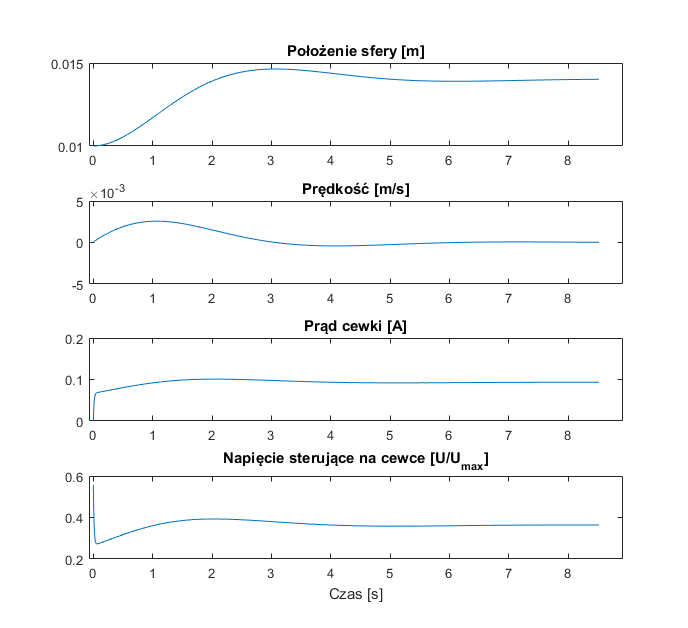
\includegraphics[scale=0.85]{img/model_LQR_stabilizacja.png}
\caption{Stabilizacja modelu nieliniowego MagLev regulatorem LQ dla modelu zlinearyzowanego wokół stanu ustalonego 14 mm}
\label{img:model_LQR}
\end{figure}





